%%%%%%%%%%%%%%%%%%%%%%%%%%%%%%%%%%%%%%%%%
% Beamer Presentation
% LaTeX Template
% Version 1.0 (10/11/12)
%
% This template has been downloaded from:
% http://www.LaTeXTemplates.com
%
% License:
% CC BY-NC-SA 3.0 (http://creativecommons.org/licenses/by-nc-sa/3.0/)
%
%%%%%%%%%%%%%%%%%%%%%%%%%%%%%%%%%%%%%%%%%

%----------------------------------------------------------------------------------------
%	PACKAGES AND THEMES
%----------------------------------------------------------------------------------------

\documentclass{beamer}

%% \mode<presentation> {

% The Beamer class comes with a number of default slide themes
% which change the colors and layouts of slides. Below this is a list
% of all the themes, uncomment each in turn to see what they look like.

%\usetheme{default}
%\usetheme{AnnArbor}
%\usetheme{Antibes}
%\usetheme{Bergen}
%\usetheme{Berkeley}
%\usetheme{Berlin}
%\usetheme{Boadilla}
%\usetheme{CambridgeUS}
%\usetheme{Copenhagen}
%\usetheme{Darmstadt}
%\usetheme{Dresden}
%\usetheme{Frankfurt}
%\usetheme{Goettingen}
%\usetheme{Hannover}
%\usetheme{Ilmenau}
%\usetheme{JuanLesPins}
%\usetheme{Luebeck}
\usetheme{Madrid}
%% \usetheme{Malmoe}
%\usetheme{Marburg}
%\usetheme{Montpellier}
%% \usetheme{PaloAlto}
%\usetheme{Pittsburgh}
%\usetheme{Rochester}
%\usetheme{Singapore}
%\usetheme{Szeged}
%% \usetheme{Warsaw}

% As well as themes, the Beamer class has a number of color themes
% for any slide theme. Uncomment each of these in turn to see how it
% changes the colors of your current slide theme.

%\usecolortheme{albatross}
%\usecolortheme{beaver}
%\usecolortheme{beetle}
%\usecolortheme{crane}
%\usecolortheme{dolphin}
%\usecolortheme{dove}
%\usecolortheme{fly}
%\usecolortheme{lily}
%\usecolortheme{orchid}
%\usecolortheme{rose}
%\usecolortheme{seagull}
%\usecolortheme{seahorse}
%\usecolortheme{whale}
%\usecolortheme{wolverine}

%\setbeamertemplate{footline} % To remove the footer line in all slides uncomment this line
%% \setbeamertemplate{footline}[page number] % To replace the footer line in all slides with a simple slide count uncomment this line

\setbeamertemplate{navigation symbols}{} % To remove the navigation symbols from the bottom of all slides uncomment this line
%% }

% Language and fonts
\usepackage[T2A]{fontenc}
\usepackage[utf8]{inputenc}
\usepackage[english,russian]{babel}

\usepackage{fontspec}
\setmainfont[Ligatures={TeX,Historic}]{Liberation Serif}
\setsansfont{Liberation Sans}
\setmonofont{Liberation Mono}
\usefonttheme{professionalfonts}
\usefonttheme{serif}

% References
\usepackage[
    backend=biber,
    bibencoding=utf8,
    sorting=none,
    sortcites=true,
    bibstyle=gost-numeric,
    citestyle=authortitle-ticomp,
    autolang=other
]{biblatex}

\usepackage{graphicx} % Allows including images
\usepackage{booktabs} % Allows the use of \toprule, \midrule and \bottomrule in tables
\usepackage{appendixnumberbeamer}

\DeclareMathOperator{\argmin}{argmin}
\DeclareMathOperator{\argmax}{argmax}

% Footcites in columns
\addtobeamertemplate{footnote}{\vspace{-6pt}\advance\hsize-0.5cm}{\vspace{6pt}}
\makeatletter
% Alternative A: footnote rule
\renewcommand*{\footnoterule}{\kern -3pt \hrule \@width 2in \kern 8.6pt}
% Alternative B: no footnote rule
% \renewcommand*{\footnoterule}{\kern 6pt}
\makeatother

\addbibresource{master-thesis.bib}

%----------------------------------------------------------------------------------------
%	TITLE PAGE
%----------------------------------------------------------------------------------------

% The short title appears at the bottom of every slide, the full title is only on the title page
\title[DQN-routing]{
  Децентрализованный алгоритм управления конвейерной системой
  с использованием методов мультиагентного обучения с подкреплением
}

\author[Дмитрий Мухутдинов, М4239]{
  Мухутдинов Дмитрий, группа M4239 \\
  Научный руководитель: Фильченков А. А., к.ф-м.н., доцент ФИТиП \\
  Консультант: Вяткин В.В., д.т.н., профессор ФИТиП
}% Your name
\institute[ИТМО] % Your institution as it will appear on the bottom of every slide, may be shorthand to save space
{
  Факультет Информационных Технологий и Программирования \\
  Мегафакультет Трансляционных Информационных Технологий \\
  Университет ИТМО, Санкт-Петербург
}
\date{\today} % Date, can be changed to a custom date

\graphicspath{{img/}}

\begin{document}

\frame{\titlepage}

%----------------------------------------------------------------------------------------
%	PRESENTATION SLIDES
%----------------------------------------------------------------------------------------

\begin{frame}
  \frametitle{Конвейерные системы}
  Применения:
  \begin{itemize}
  \item Промышленность
  \item Сортировка грузов
  \item Распределение багажа
  \item ...
  \end{itemize}
  Будем рассматривать случай с багажом.
\end{frame}

%------------------------------------------------

\begin{frame}
  \frametitle{Существующие решения}
  \begin{itemize}
  \item Статические стратегии управления\footcite{de1994baggage}
    \begin{itemize}
    \item Разрабатываются под конкретную топологию системы
    \end{itemize}
  \item Model predictive control (MPC)\footcite{cataldo2016dynamic}\footcite{zeinaly2015integrated}\footcite{luo2015energy}
    \begin{itemize}
    \item Решает глобальную оптимизационную задачу в форме LP/QP
    \item Вся система контролируется централизованно
    \item Не может обрабатывать изменения в системе, не заложенные в модель (поломки)
    \end{itemize}
  \item Маршрутизация по аналогии с компьютерными сетями\footcite{vyatkin-controllers}
    \begin{itemize}
    \item Децентрализованное вычисление, устойчивость к поломкам
    \item Оптимизирует только скорость доставки чемоданов
    \end{itemize}
  \end{itemize}
\end{frame}

%------------------------------------------------

\begin{frame}
  \frametitle{Цель работы}
  Разработать алгоритм управления конвейерной системой со следующими свойствами:
  \begin{itemize}
  \item Децентрализованность
  \item Многокритериальная оптимизация (время доставки багажа +
    энергопотребление)
  \item Устойчивость к разнородным изменениям в условиях среды
    \begin{itemize}
    \item Изменения характеристик багажного потока
    \item Поломки конвейеров
    \end{itemize}
  \end{itemize}
\end{frame}

%-------------------------------------------------

\begin{frame}
  \frametitle{Идея}
  \begin{itemize}
  \item Сосредоточимся на обобщенной задаче маршрутизации в ориентированном графе
  \item Обучение с подкреплением
  \item Нейросети в качестве обучающихся агентов
  \item Q-routing\footcite{q-routing-orig}
    \begin{itemize}
    \item Не получил широкого распространения в компьютерных сетях (использует
      слишком много служебных пакетов)
    \item В других задачах (трафик, конвейеры) это не является проблемой.
    \end{itemize}
  \end{itemize}
\end{frame}

%------------------------------------------------

\begin{frame}
  \frametitle{Постановка задачи в терминах RL}
  \begin{itemize}
    \item Рассмотрим \textit{пакет} в сети как обучающегося агента,
      взаимодействующего с сетью как со средой
    \item Полное состояние среды неизвестно, состояние текущего роутера ---
      \textit{наблюдение} пакета
    \item Действие --- переход к одному из соседей
    \item Q-learning:
      \[
      Q(o_t, a_t) \leftarrow r_t + \gamma \cdot
      \max\limits_{a \in \mathcal{A}_{o_{t+1}}} {Q(o_{t+1}, a)}
      \]
    \item Принцип аналогичный Q-routing:
      \[
      Q_x(d, y) \leftarrow (t_{finish} - t_{start}) +
      \max\limits_{z \in \{ V | (y, z) \in E\}} {Q_y(d, z)}
      \]
  \end{itemize}
\end{frame}

%----------------------------------------------------------------

\begin{frame}
  \frametitle{Что было сделано}
  \begin{columns}
    \begin{column}{0.5\textwidth}
      Алгоритм DQN-routing\footnotemark
      \begin{itemize}
      \item Объединяет link-state протокол с алгоритмом Q-routing
      \item Вход нейросети:
        \begin{itemize}
        \item Номер текущего узла
        \item Номер узла назначения
        \item Узлы-соседи
        \item Матрица смежности графа
        \end{itemize}
      \end{itemize}
      Был протестирован в сеттинге компьютерных и конвейерных сетей
    \end{column}
    \begin{column}{0.5\textwidth}
      \begin{center}
        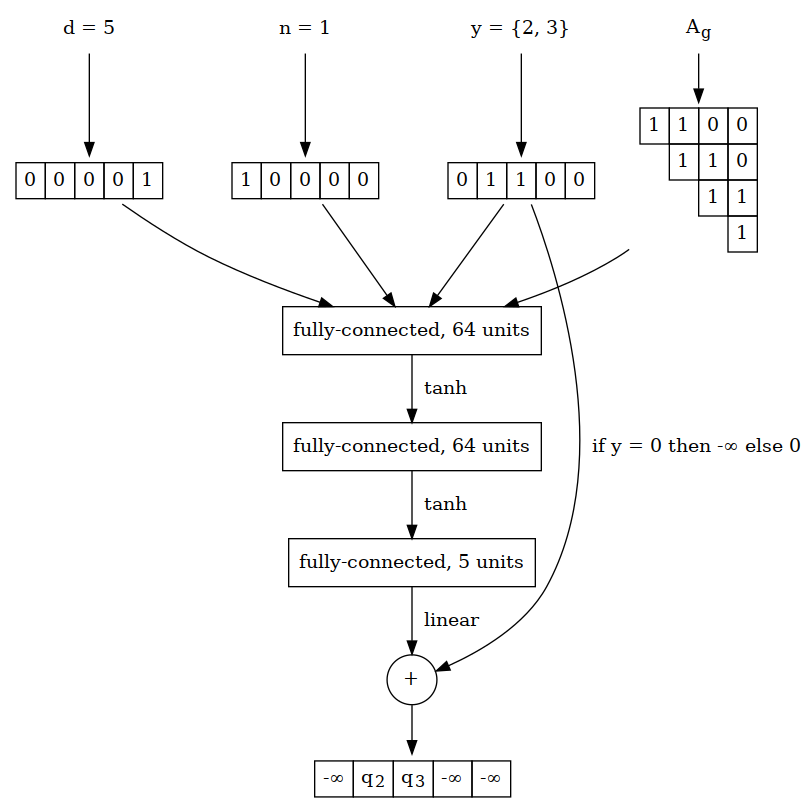
\includegraphics[width=\textwidth]{nn-2}
      \end{center}
    \end{column}
  \end{columns}
  \footcitetext{mukhutdinov2019multi}
\end{frame}

\begin{frame}
  \frametitle{Эксперименты в модели компьютерной сети}
  \begin{columns}
    \begin{column}{0.6\textwidth}
      \begin{itemize}
      \item Запуск экспериментов в симуляторе
      \item Сравнение архитектур между собой и сравнение с алгоритмами link-state и Q-routing
      \item Служебные сообщения доставляются бесплатно
      \end{itemize}
    \end{column}
    \begin{column}{0.4\textwidth}
      \begin{center}
        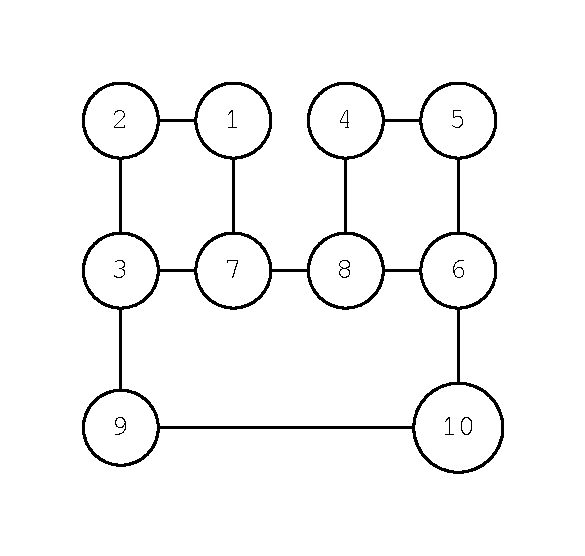
\includegraphics[width=0.7\textwidth]{graph-2}

        Топология сети для тестов
      \end{center}
    \end{column}
  \end{columns}
\end{frame}

%------------------------------------------------------

\begin{frame}
  \frametitle{Изменение топологии сети: сравнение с link-state и Q-routing}
  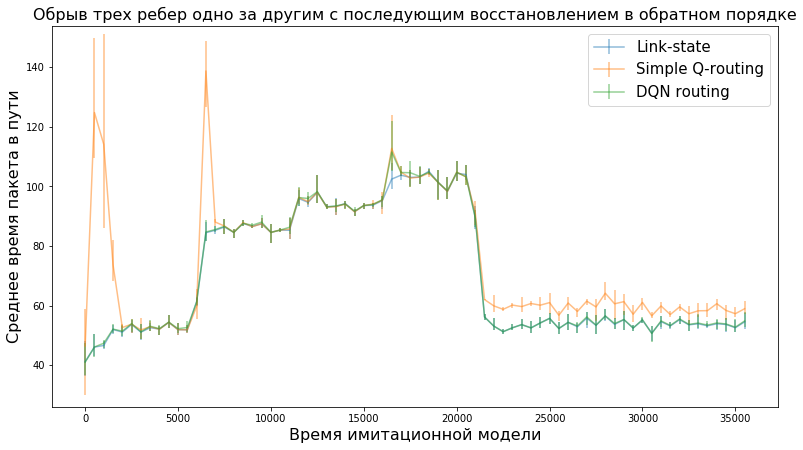
\includegraphics[width=\textwidth]{experiment-link-failures} 
\end{frame}

%------------------------------------------------------

\begin{frame}
  \frametitle{Изменение нагрузки: сравнение c link-state и Q-routing}
  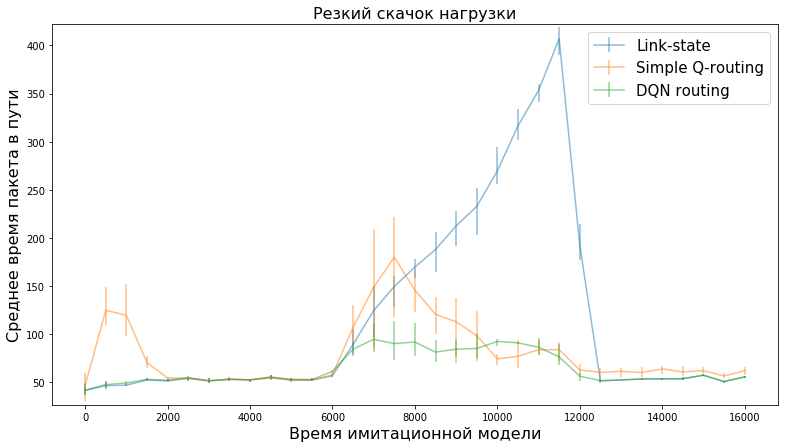
\includegraphics[width=\textwidth]{experiment-peak-load} 
\end{frame}

%------------------------------------------------------

\begin{frame}
  \frametitle{Эксперименты в модели системы багажных конвейеров}
  \begin{columns}
    \begin{column}{0.5\textwidth} 
      \begin{itemize}
      \item Конвейерная сеть моделируется как ориентированный граф
      \item Каждая секция конвейера -- отдельная вершина
      \item В оптизируемую функцию включено \textit{энергопотребление}
      \item На вход нейросети дополнительно подается информация о состоянии конвейеров
      \item Важность экономии энергии регулируется параметром $\alpha$
      \end{itemize}
    \end{column}
    \begin{column}{0.5\textwidth}
      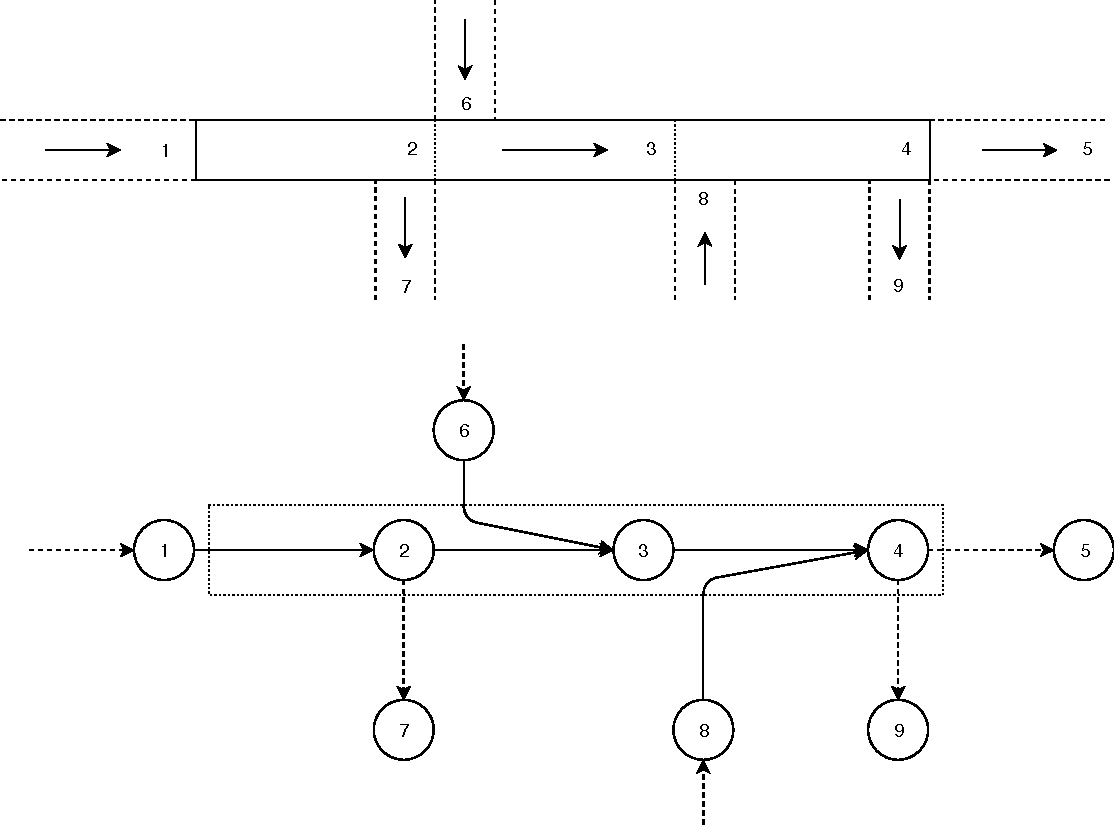
\includegraphics[width=\textwidth]{belt-illustration}  

      Участок конвейерной сети и соответствующий участок графа
    \end{column}
  \end{columns}
\end{frame}

%------------------------------------------------------

\begin{frame}
  \frametitle{Модель конвейерной системы для проведения экспериментов}
  \begin{center}
    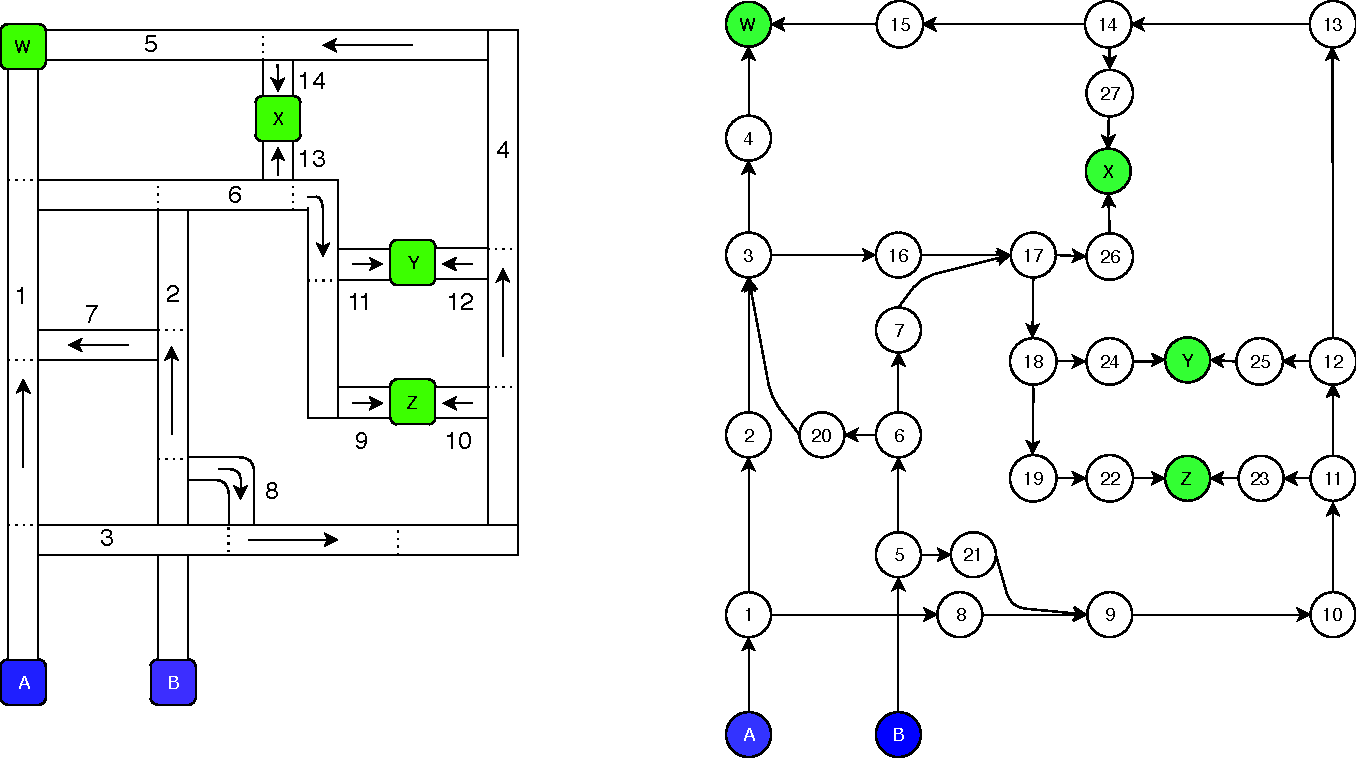
\includegraphics[width=0.9\textwidth]{test-conveyors} 
  \end{center}
\end{frame}

%------------------------------------------------------

\begin{frame}
  \frametitle{Неравномерный поток до выходных вершин: сравнение c link-state и Q-routing}
  \begin{columns}
    \begin{column}{0.5\textwidth}
      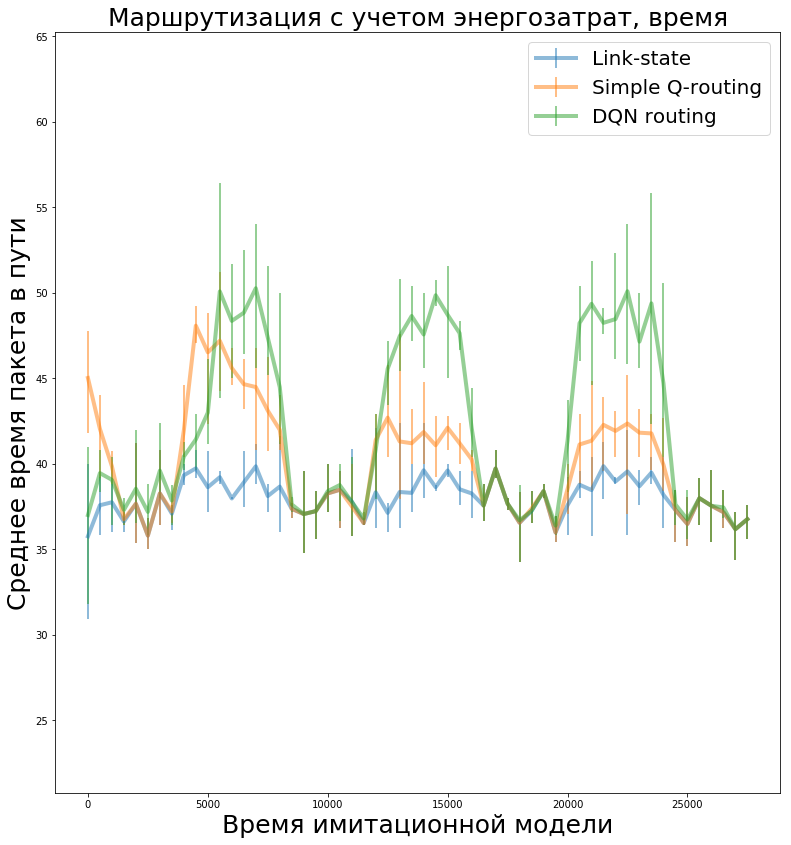
\includegraphics[width=\textwidth]{experiment-conveyors-en1-time-tall}
    \end{column}
    \begin{column}{0.5\textwidth}
      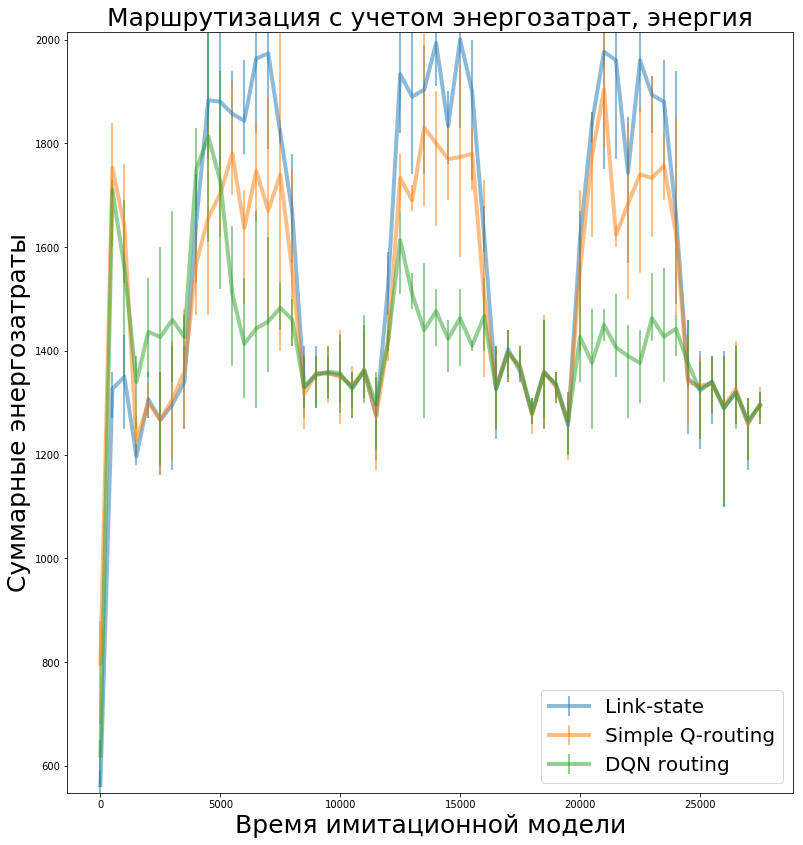
\includegraphics[width=\textwidth]{experiment-conveyors-en1-energy-tall}
    \end{column}
  \end{columns}
\end{frame}

%------------------------------------------------------

\begin{frame}
  \frametitle{Плавное повышение нагрузки: $\alpha = 1$}
  \begin{columns}
    \begin{column}{0.5\textwidth}
      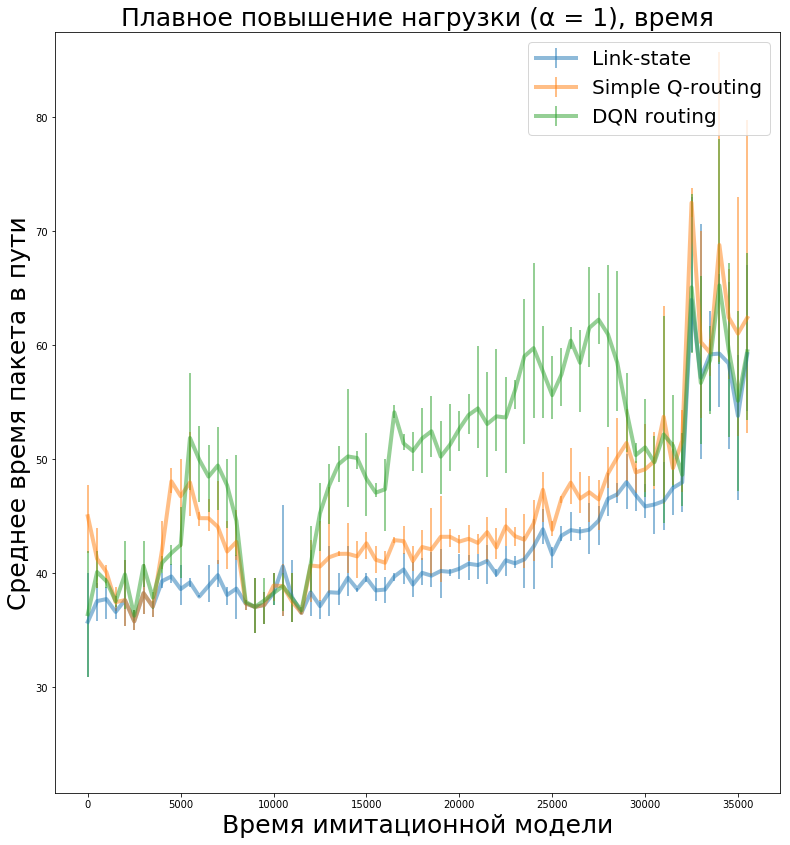
\includegraphics[width=\textwidth]{experiment-conveyors-a1-time-tall}
    \end{column}
    \begin{column}{0.5\textwidth}
      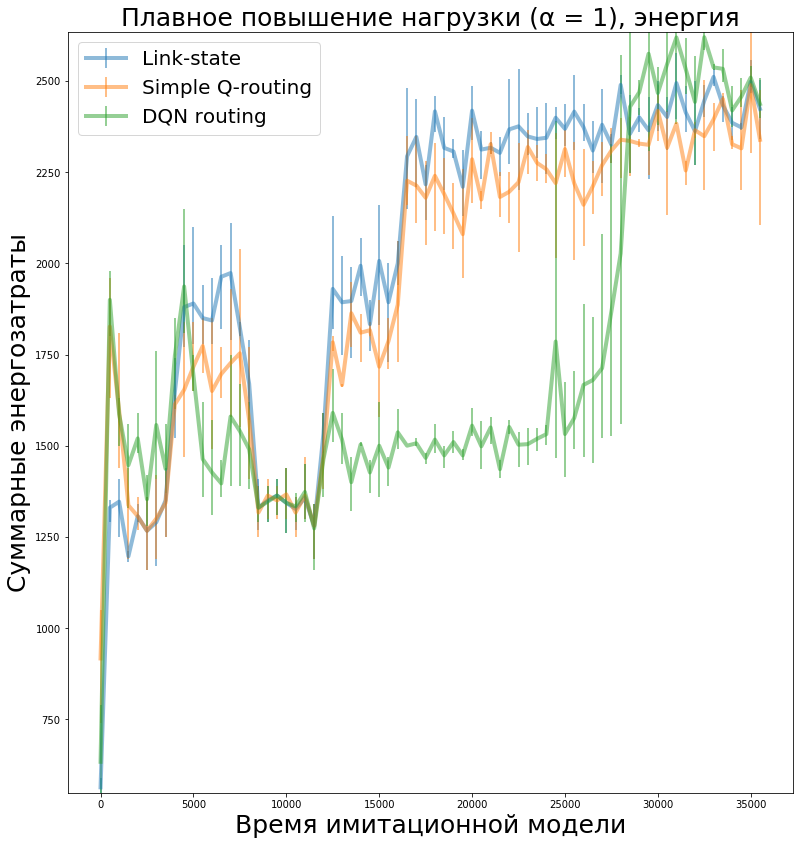
\includegraphics[width=\textwidth]{experiment-conveyors-a1-energy-tall}
    \end{column}
  \end{columns}
\end{frame}

%------------------------------------------------------

\begin{frame}
  \frametitle{Плавное повышение нагрузки: $\alpha = 0.6$}
  \begin{columns}
    \begin{column}{0.5\textwidth}
      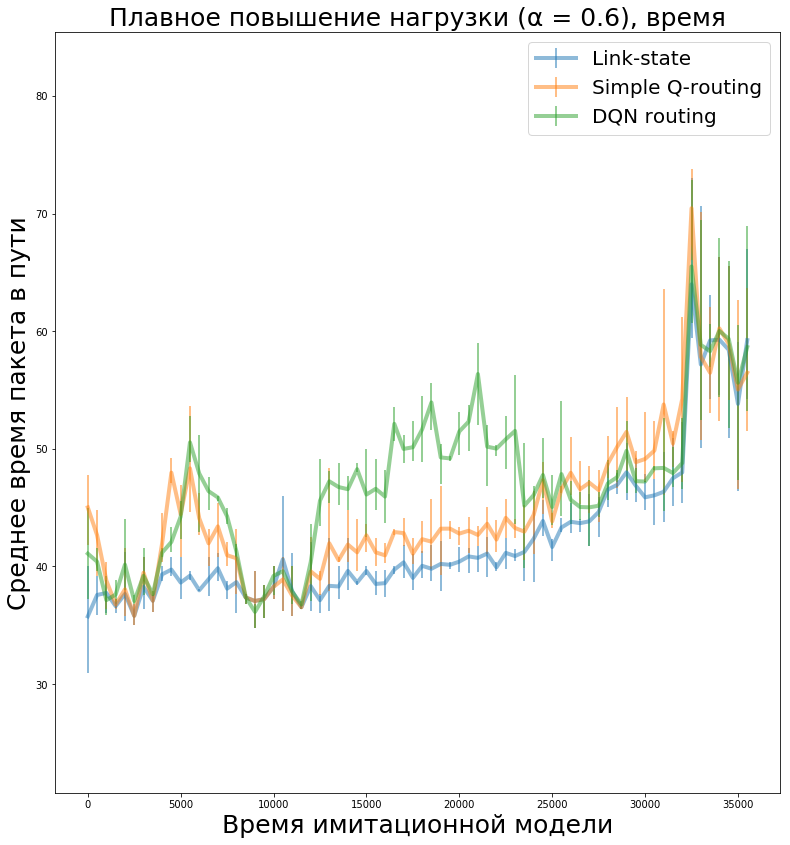
\includegraphics[width=\textwidth]{experiment-conveyors-a06-time-tall}
    \end{column}
    \begin{column}{0.5\textwidth}
      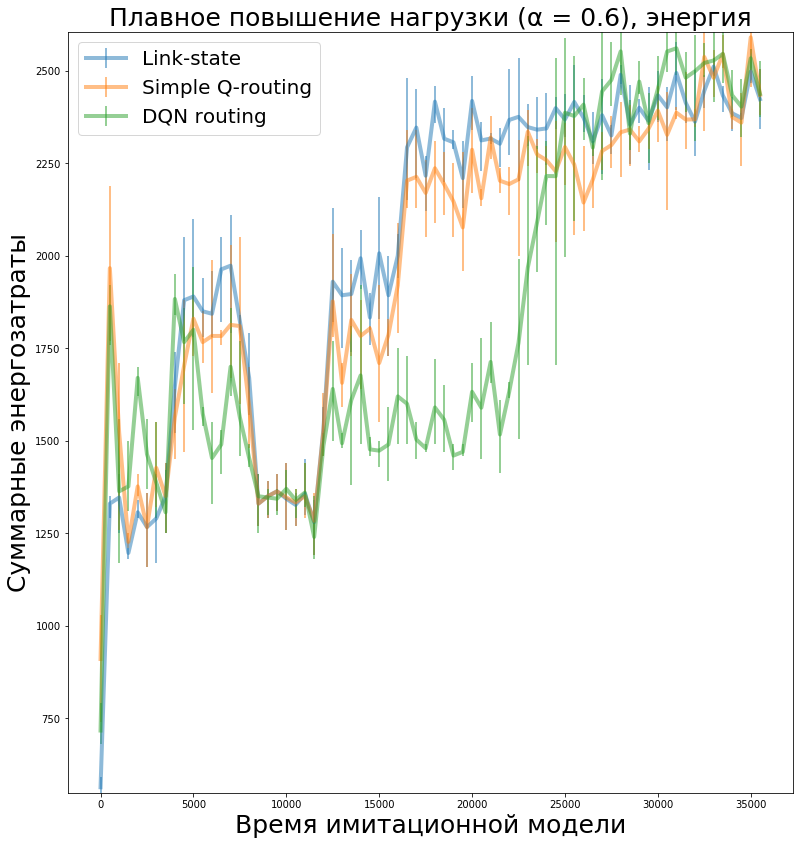
\includegraphics[width=\textwidth]{experiment-conveyors-a06-energy-tall}
    \end{column}
  \end{columns}
\end{frame}

%-------------------------------------------------------

\begin{frame}
  \frametitle{Плюсы и минусы DQN-routing}
  \begin{itemize}
  \item Плюсы
    \begin{itemize}
    \item Адаптация под изменения трафика
    \item Адаптация после поломок
    \item Оптимизация времени доставки и энергопотребления с заданным приоритетом
    \end{itemize}
  \item Минусы
    \begin{itemize}
    \item Размер выходного слоя линейно зависит от размера графа
    \item Размер входного слоя квадратично зависит от размера графа
    \item Требует предварительного обучения с учителем
    \end{itemize}
  \end{itemize}
\end{frame}

%-------------------------------------------------------

\begin{frame}
  \frametitle{Идеи усовершенствования алгоритма}
  \begin{itemize}
  \item Предсказание Q-функции отдельно для каждого исходящего ребра
  \item Использование графовых эмбеддингов
  %% \item Использование метода актора-критика
  \item Зональная маршрутизация
  \item Построение глобальной графовой нейронной сети (GG-NN)
  \end{itemize}
\end{frame}

%-------------------------------------------------------

\begin{frame}
  \frametitle{Предсказание Q-функции для соседей по отдельности}
  \begin{columns}
    \begin{column}{0.6\textwidth}
      \begin{itemize}
      \item Только небольшое количество узлов в сети являются нашими соседями по
        исходящим ребрам
      \item Можем предсказывать значение Q-функции для каждого из них в
        отдельности, подавая номер каждого из них на вход
      \item Избавляемся от линейной зависимости размера выходного слоя от
        размера графа
      \item Качество работы остается прежним
      \end{itemize}
    \end{column}
    \begin{column}{0.4\textwidth}
      \begin{center}
        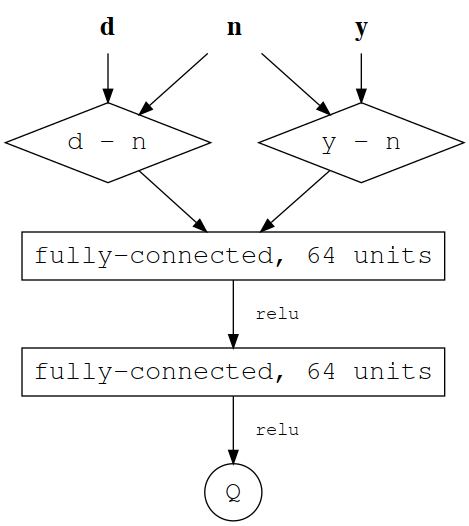
\includegraphics[width=\textwidth]{nn-1-one-out}
      \end{center}
    \end{column}
  \end{columns}
\end{frame}

\begin{frame}
  \frametitle{Иcпользование графовых эмбеддингов: идея}
  \begin{itemize}
  \item Вместо кодирования меток узлов унитарным кодом использовать их
    отображения в векторное пространство фиксированной размерности
  \item Отказ от подачи на вход матрицы смежности
    \begin{itemize}
      \item Вместо этого пересчитывать эмбеддинги при изменении топологии
      \item Эмбеддинги косвенно передадут информацию о топологии
    \end{itemize}
  \end{itemize}
\end{frame}

%% \begin{frame}
%%   \frametitle{Иcпользование графовых эмбеддингов: результаты}
%%   Алгоритм HOPE\footcite{ou2016asymmetric} с использованием Katz index как
%%   метрики похожести.
%%   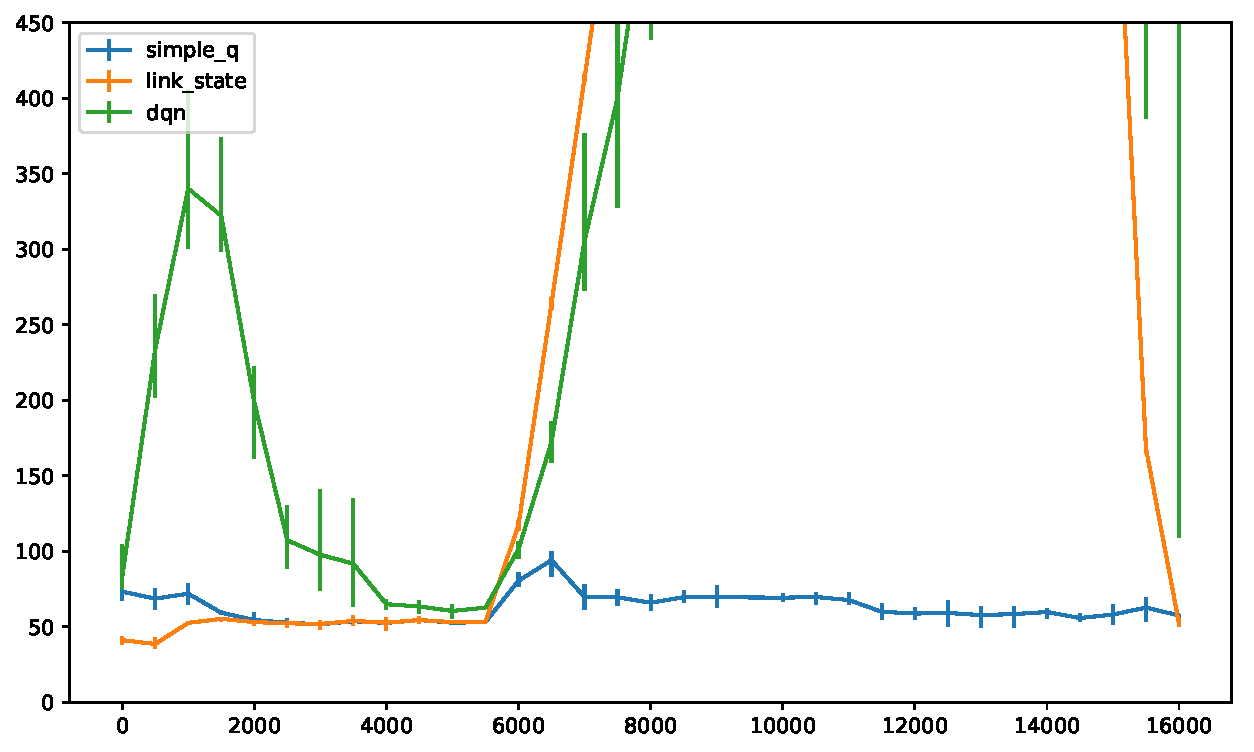
\includegraphics[width=0.8\textwidth]{peak-load-embedding} \\
%%   :(
%% \end{frame}

%-------------------------------------------------------

\begin{frame}
  \frametitle{Зональная маршрутизация: идея}
  \begin{columns}
    \begin{column}{0.6\textwidth}
      \begin{itemize}
      \item Ограничиваем рассматриваемый граф только узлами не далее $k$ ребер от
        данного 
      \item Если узел назначения находится вне текущей зоны --- делаем запрос к
        узлам на границе зоны.
      \end{itemize}
    \end{column}
    \begin{column}{0.4\textwidth}
      \begin{center}
        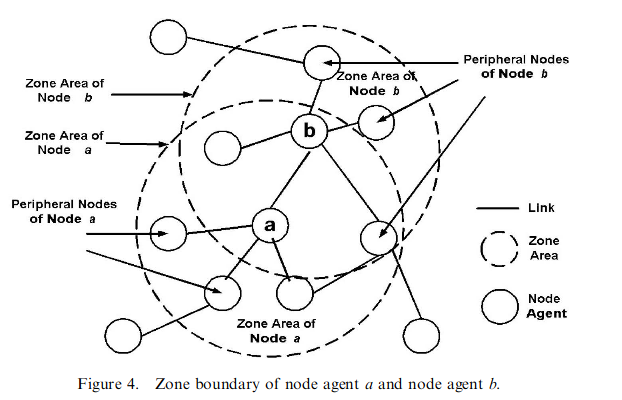
\includegraphics[width=\textwidth]{zone-routing}
      \end{center}
    \end{column}
  \end{columns}
\end{frame}

%% \begin{frame}
%%   \frametitle{Зональная маршрутизация: результаты}
%%   \huge{:shrug:}
%% \end{frame}

%-------------------------------------------------------

\begin{frame}
  \frametitle{Глобальная графовая нейронная сеть: идея}
  \begin{columns}
    \begin{column}{0.6\textwidth}
      \begin{itemize}
      \item Рассматриваем весь граф с состояниями ребер и узлов как вход для
        графовой нейронной сети (GG-NN)
      \item Считается распределенно на физических узлах системы
      \item Промежуточные состояния и их градиенты передаются между узлами по
        сети 
        \begin{itemize}
        \item Применяется для компьютерных сетей с обучением с учителем\footnotemark
        \item Добавим обучение с подкреплением во время работы
        \end{itemize} 
      \end{itemize}
    \end{column}
    \begin{column}{0.4\textwidth}
      \begin{center}
        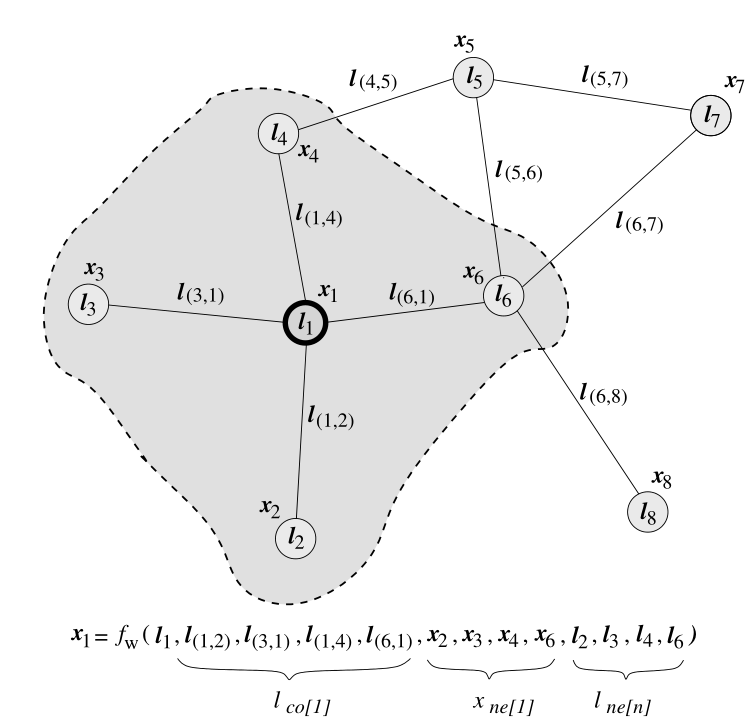
\includegraphics[width=\textwidth]{gnn.png}
        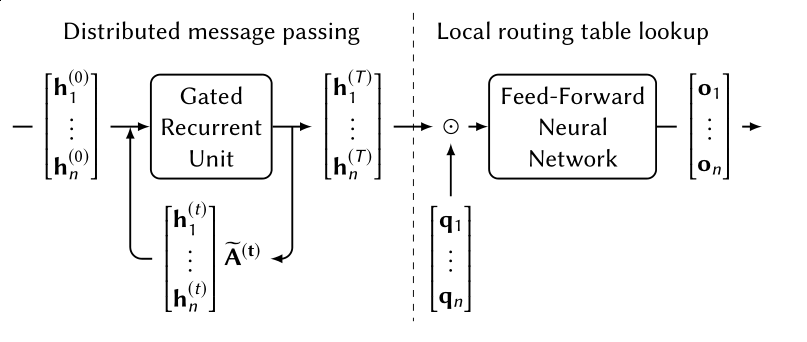
\includegraphics[width=\textwidth]{gg-qnn.png}
      \end{center}
    \end{column}
  \end{columns}
  \footcitetext{geyer2018learning}
\end{frame}

%% \begin{frame}
%%   \frametitle{Глобальная графовая нейронная сеть: результаты}
%%   \huge{:shrug:}
%% \end{frame}

%-------------------------------------------------------

%% \begin{frame}
%%   \frametitle{Итоги}
%%   \begin{itemize}
%%   \item :shrug:
%%   \end{itemize}
%% \end{frame}

%-------------------------------------------------------

\begin{frame}
  \frametitle{Прочие направления дальнейших исследований}
  \begin{itemize}
  \item Проведение большего числа экспериментах на различных топологиях
  \item Динамическое управление скоростями конвейеров
  \end{itemize}
\end{frame}

%-------------------------------------------------------

\begin{frame}
  \begin{center}
    {\Huge Спасибо за внимание!}
  \end{center}
\end{frame}

%% \begin{frame}[allowframebreaks]
%%   \frametitle{Библиография}
%%   \printbibliography
%% \end{frame}

%-------------------------------------------------------
%% \appendix

%% \begin{frame}
%%   \frametitle{Иллюстрация несходимости алгоритма к оптимуму без предобучения}
%%   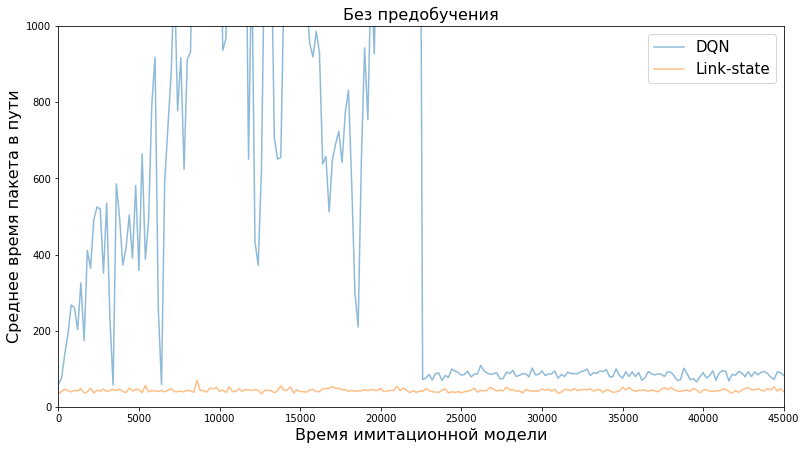
\includegraphics[width=\textwidth]{non-convergence}
%% \end{frame}

%% \begin{frame}
%%   \frametitle{Сравнение алгоритмов оптимизации: скорость предобучения}
%%   \begin{columns}
%%     \begin{column}{0.5\textwidth}
%%       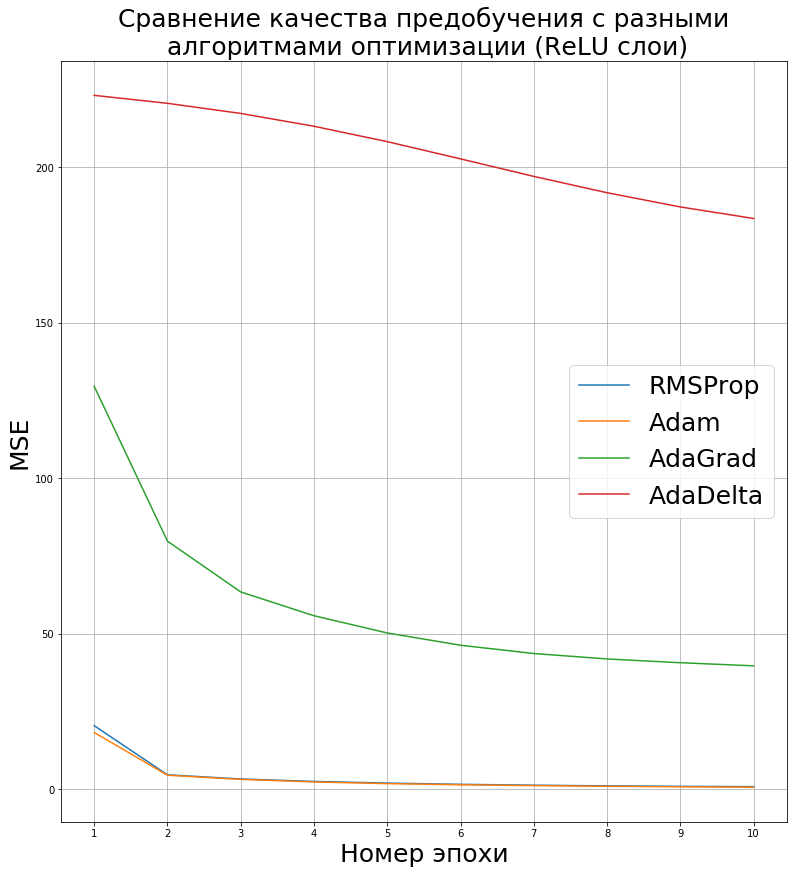
\includegraphics[width=\textwidth]{experiment-optimizers-pretrain-tall}
%%     \end{column}
%%     \begin{column}{0.5\textwidth}
%%       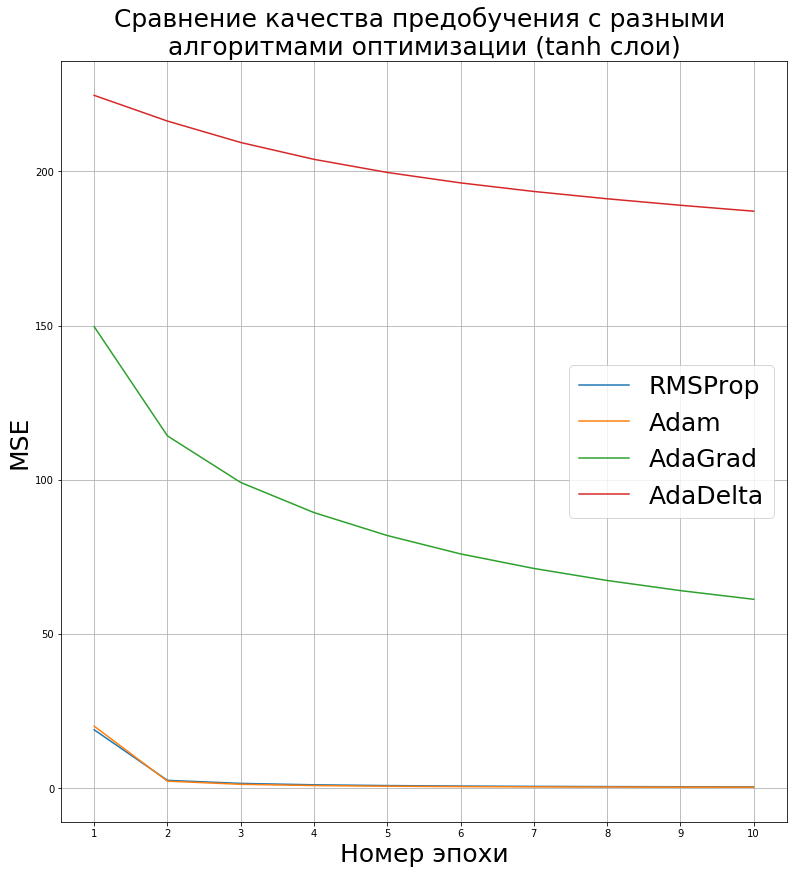
\includegraphics[width=\textwidth]{experiment-optimizers-pretrain-tanh-tall}
%%     \end{column}
%%   \end{columns}
%% \end{frame}

%% \begin{frame}
%%   \frametitle{Сравнение алгоритмов оптимизации и функций активации: скорость предобучения}
%%   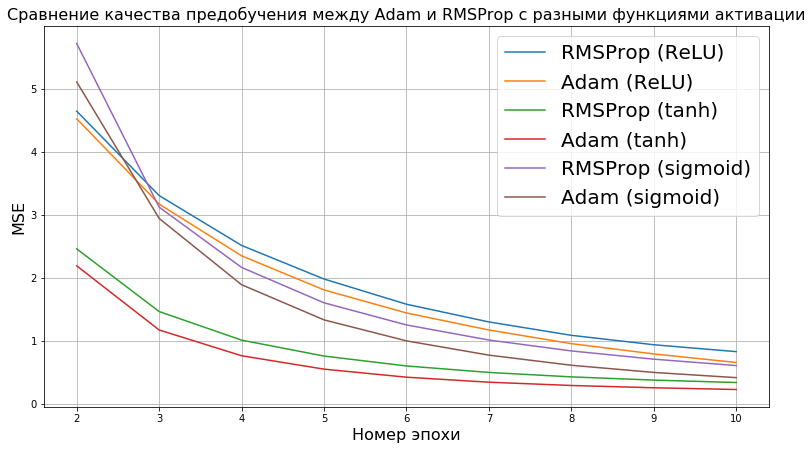
\includegraphics[width=\textwidth]{experiment-optimizers-pretrain-adam-vs-rmsprop}
%% \end{frame}

%% \begin{frame}
%%   \frametitle{Сравнение RMSProp и Adam в модели компьютерной сети}
%%   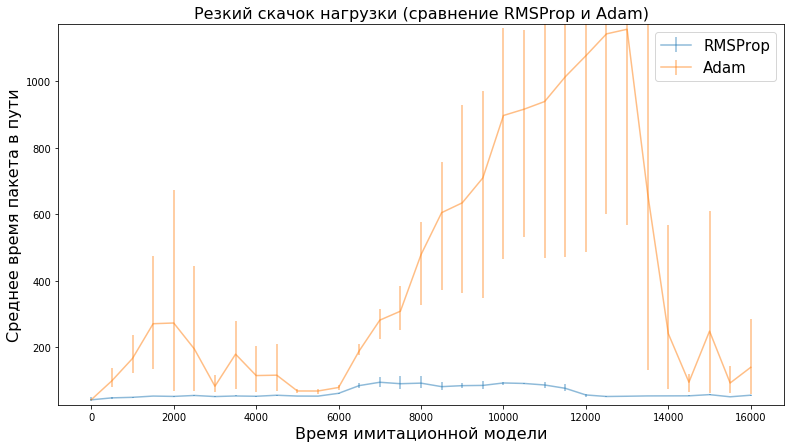
\includegraphics[width=\textwidth]{experiment-adam-failure}
%% \end{frame}

%% \begin{frame}
%%   \frametitle{Сравнение фукнций активации c RMSProp в модели компьютерной сети}
%%   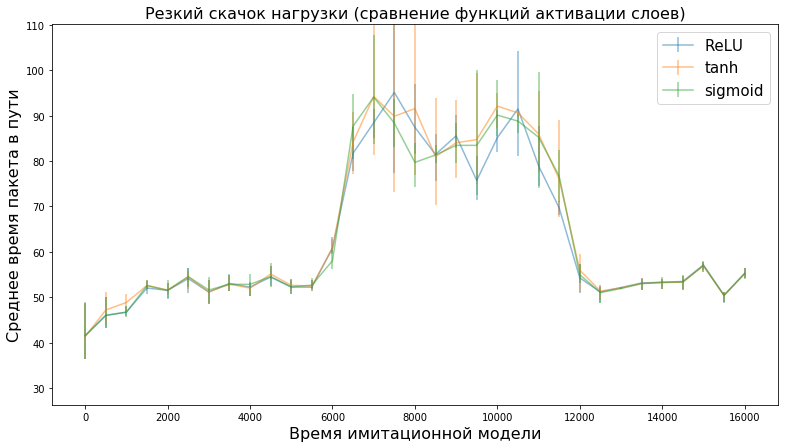
\includegraphics[width=\textwidth]{experiment-activations-launch}
%% \end{frame}

%% \begin{frame}
%%   \frametitle{Сравнение различных конфигураций feed-forward нейросети по
%%     качеству предобучения}
%%   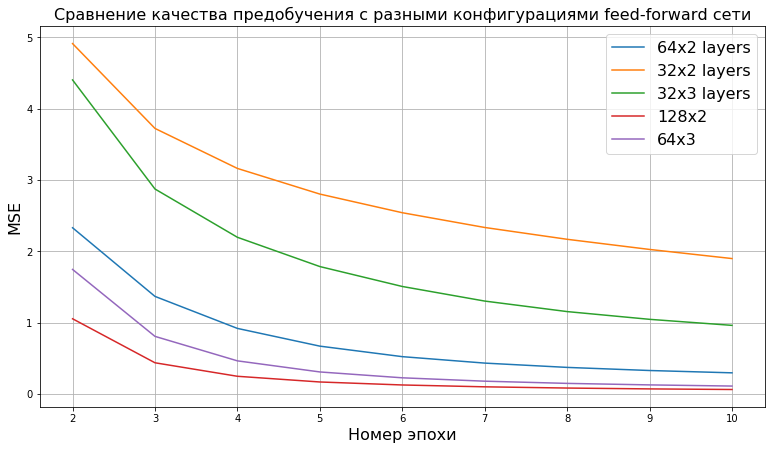
\includegraphics[width=\textwidth]{experiment-layers-pretrain}
%% \end{frame}

%% \begin{frame}
%%   \frametitle{Сравнение различных конфигураций feed-forward нейросети при работе
%%     в имитационной модели}
%%   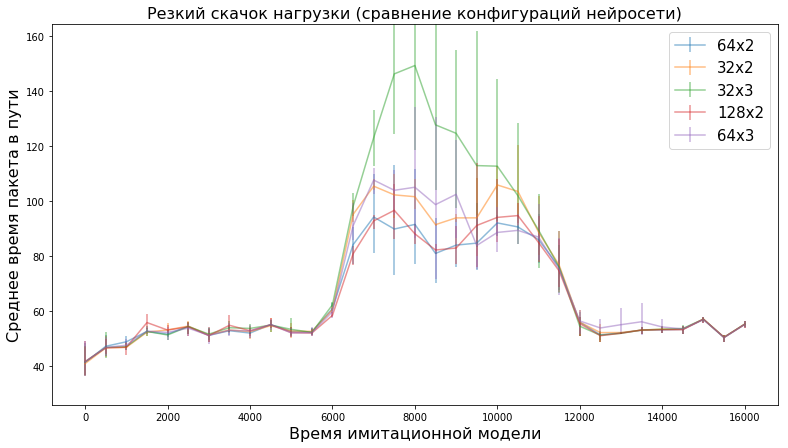
\includegraphics[width=\textwidth]{experiment-layers-launch}
%% \end{frame}

%% \begin{frame}
%%   \frametitle{Влияние softmax-стратегии на работу алгоритма}
%%   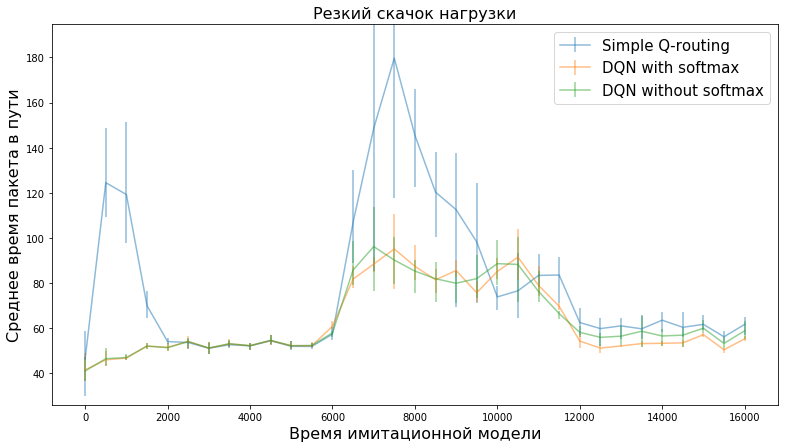
\includegraphics[width=\textwidth]{experiment-softmax-effect}
%% \end{frame}

%% \begin{frame}
%%   \frametitle{Влияние различных видов experience replay на работу алгоритма}
%%   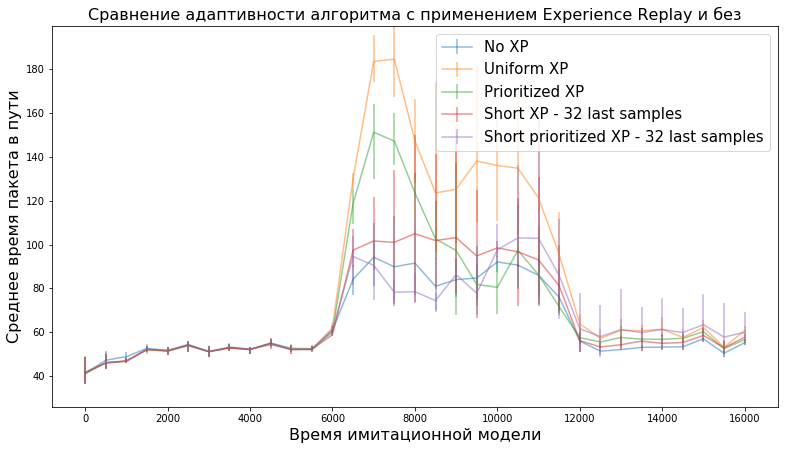
\includegraphics[width=\textwidth]{experiments-xp-variants}
%% \end{frame}

%% \begin{frame}
%%   \frametitle{Влияние включения матрицы смежности в наблюдаемое состояние}
%%   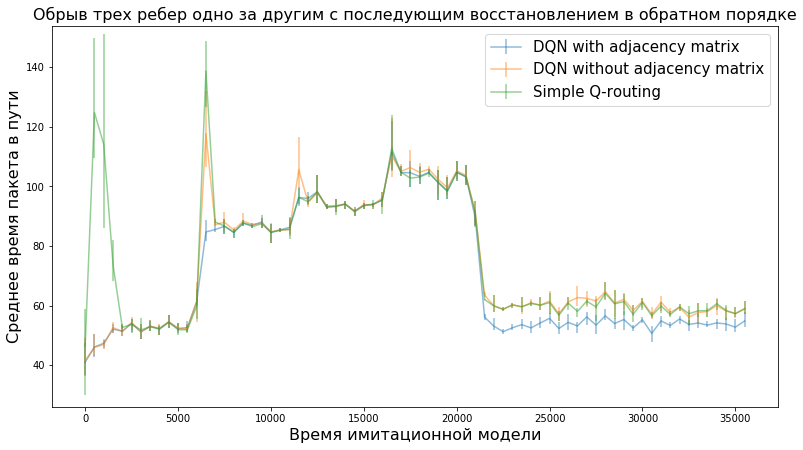
\includegraphics[width=\textwidth]{experiment-with-without-amatrix}
%% \end{frame}

%% \begin{frame}
%%   \frametitle{Влияние включения информации о состоянии соседних конвейеров в
%%     наблюдаемое состояние}
%%   \begin{columns}
%%     \begin{column}{0.5\textwidth}
%%       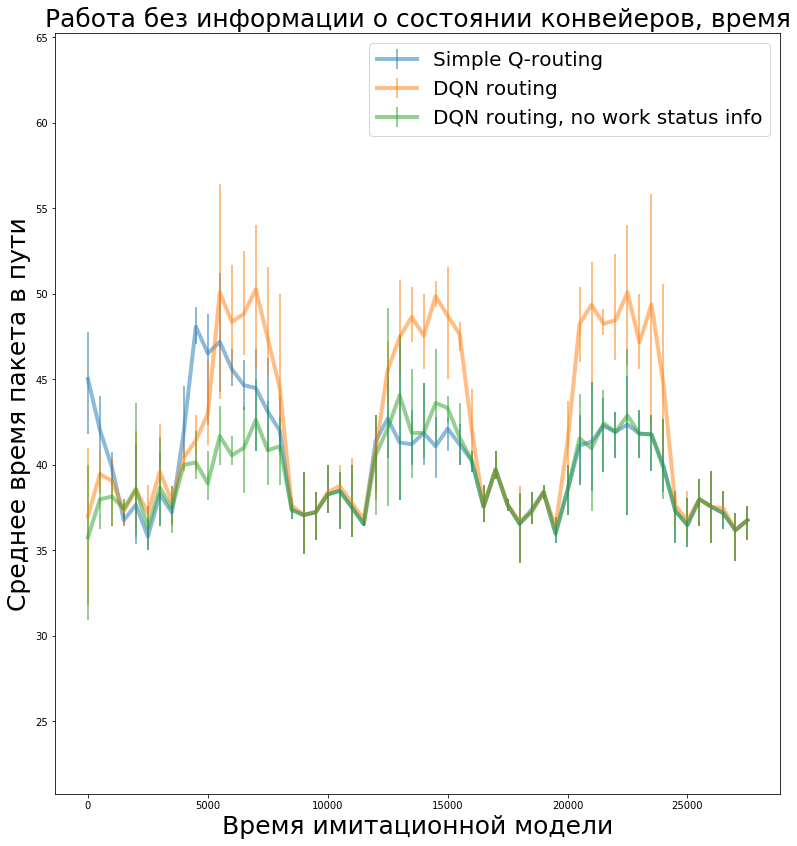
\includegraphics[width=\textwidth]{experiment-conveyors-en1-time-no-ws-tall}
%%     \end{column}
%%     \begin{column}{0.5\textwidth}
%%       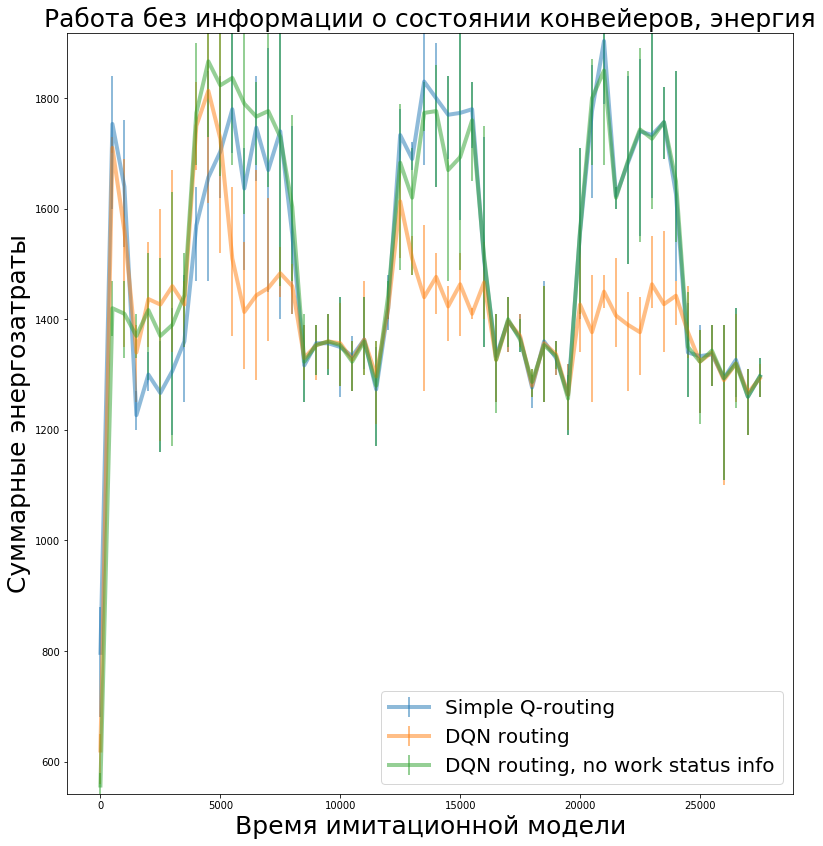
\includegraphics[width=\textwidth]{experiment-conveyors-en1-energy-no-ws-tall}
%%     \end{column}
%%   \end{columns}
%% \end{frame}

\end{document} 
